\hmsubsection{Test Setup}{FKT}{}

Implementation of testing process have been systematic and applied different procedures to verify that the robot arm meets the desired specifications, such as reliable overall performance and operational safety in real time phase. The validation confirmed systems operation across sensor and environmental interpretation, communication of command-and-control system using OpenRB-150, Raspberry pi and mechanical system. The purpose of testing set up has ensured efficient integration and optimal performance of the robot arm. We made decision system that before we dive in any integration test the system must approve in isolated test set up including technical and conceptual system setting up precisely and completely. This is a framework within the context of avoiding false integration failures minimizing discovering invisible limitations. Low level setup allowed us to find out isolated error or mistaken defect error both technical and system base.




During component tests we encountered motor defects where we initially thought two out of three servo motors were defects. In the meantime, due to the first mentioned test mechanism, we applied all motors tested again and were false defect. This led us to believe that low level setup such as technical test setup would be critical for systems integration test. This test setup described here has been conducted to be unequivocal for components condition both hardware and software units. The method has been effective in system configuration specifically for calibration of OpenRB-150 and Raspberry pi units along with software model configuration. Further the procedure advanced to execute on robust integration test for the two layers. The first integration testing layer that handled the verification of interfaces between subsystems. Secondly the verification and validation layer that confirmed robot arm integration meets the design specification and operational requirement expected to fulfill. 



Set up Camera 

The camera in place implementation camera set up by the OAK-D S2 camera served as eye for the robot arm designated with the lens pointed at the conveyor to gripe area from the angle specified in the robot claw tied. The sensor(camera) position is determined and is critical aspect of the lighting for sorting accuracy. Camera set up has been fundamental due to rotation translation matrix maps pixels coordinated. The camera fixed physical located relative to the conveyor to grip balls area due to transformed image pixels data into real time has been Valid test setup. In initial setup test alignment camera placed caused invalidation that led to errors in the ball’s recognition. 



The camera operated with lens captured images lighting reflected from balls on the conveyor belt with location focused on the balls image sensor. This fundamental setup has verified where the captured images of the balls convert into digital image data that ensured for reliable detection. During initial calibration phase camera with robot arm confirmed that sensor depended on correct extrinsic calibration to interpret the 3D position balls related to the robot arm. This latest test indicated the robot arm vision system achieved accurately to detect, classify and localize the balls based on their respective colors delivered precise grip and placed in the corresponding container. 



During sensor or camera performance directly influenced by lighting conditions consistent stable lighting delivered clear ball images that led effective detection. The perception algorithms received clean reliable inputs. lighting set up played crucial role in calibration, verification and balls recognition including spatial awareness. The sensor operated optimally only when secured precisely as calibrated, combined with stable controlled lighting conditions. This setup ensured the camera provided accurate spatial data for the robot arms perception and subsequent manipulation tasks.



 The set up verification camera  has been critical before any test for sorting balls. The sensor workplace calibration needs to be verified as valid for the current camera position. This objective has confirmed by placing reference balls at varied multiple positions in the lap room. These positions have been verified by once OpenRB-150 commanding the vision system successfully detected balls in all positions

 
Functional test

functional test primarily targeted ball detection progress and classification accuracy. The perception system in initial test has been volatile due to mechanical instability. During sorting in real time the robot confirmed to recognize the color classification in low level. despite a few failures on coordinated position the mechanical arm remain unstable during movement . The initial test as been held under normal lighting condition. The mechanical arm underwent through tight inspection including ability to grasp and place balls in coordinated the correct bins. In the first hand however it has been hard to comprehend where the problem precisely  existed as long as mechanical design required additional configuration. Once mechanical component of the arm designed and later integrated the next assessment seems relatively less complex to interpretation. The perception system once  again come under thorough assessment. The sensor system confirmed to recognized the color of the balls

 second test with a new mechanical arm improved in design stability. The two color classes perform below anticipation specifically blue color during initial test . The root cause was due to spectral ambiguity under different lightning. The red color under direct light instruction performed stable recognition  as near-saturated brightness across all color category. This progress ensured that the red color push nearly consistent recognition, despite a few scored below confidence threshold. According the tight observation these a few failures did not occurred due to model failure in conventional sense. The model correctly reported how the sensor measured , however it could rather the fundamental problem is observed color to physical color label during the brightness changed the obvious color of the ball.

 Perception system performance was not a fixed property of the model. It is a joint property of the model, the camera , the lighting , and the surface  characteristics of the specific balls being sorted. During systems test the position accuracy of the robot arm in real time application is essentially limited by collective errors from camera calibration, mechanical backlash and structural compliance. These layered error propagated result in higher precision near the center 



\begin{table}
\centering

\begin{tabular}{| l | l | l | l | l | l | l |}
\hline
Valid criteria & Threshold  & Red standard & Blue standard & Red Dim & Blue Dim  & system \\
\hline
Classification dim & >= 97 \% & 99 \%  & 96.0 \%  & - & - & Marginal  \\
\hline
Classification accuracy  & >= 91 \% & 0.8 \% &   &   & - & Marginal  \\
\hline
False Sort  & =< 1.8 \% &   &   &   & - & approve \\
\hline
TCP sorting error & Nuetral  & 0.9 \% &   &   & - & approve \\
\hline
Grippe failure & =< 3\% & 0.9\% & 0.9\% & - & - & Approve  \\
\hline

\end{tabular}

\end{table}

 Red balls achieved high progress in compared with blue classification across multiple environments. A few red balls due to reflection with high brightness emerged fail classification. It was routed that required light transformation by retrain the dataset for classification improvement. The blue balls has been far more environmental sensitive during real time sorting . The perception system under dim light illustrate high environment limitation. This the reason marginalized in the report above representing of the conditions 

 The role of test set up in verification and validation was essential within the robot system. The framework particularly ensure the performance where sensitivity conditions reduced to low level. The camera can encounter and the lighting transform during by opening and closing the windows. The  micro-controller unit  (OpenRB-150) can possibly flashed by accident in case of any incorrect firmware version. The perception USB belt can be replaced with different version and color. These changes would enormously challenged the result without this external indication. The prior to verification set up minimized precisely to catch certain accident that could led into unreliable conclusion.
 
 
 
 The test set up objective was not only about technical procedure, rather it was understanding the real performance of the system. The mechanism provide solid advantage on technical consistency, while ensure accelerated to understand operational  measurement that reflected how the system behaves in real environment. Ultimately, the test environment enhanced comprehensive understanding of the real operational accuracy and reliability that goes beyond technical evaluation.

operational test
operational test the direct assessment of how  the system respond under various environment. The real-time operational testing based on comprehensive data recording during sort in real time provided critical insight how the robot arm systems real performance progress. The purpose  coordinated the gap   between  h controlled offline evaluation and real time dynamic including related conventional scenarios. This mechanism accelerated 

    
 \textbf{10.3 Sorting Accuracy 
 
 }
 

The system process has been defined with stakeholders requirement on what the robot arm suppose to achieve. Our stakeholder defined the objectives and scope as this fundamental step to fulfill the requirements. The system required to sort balls according to  respective color value placed in the corresponding container position. The functional stability demanded a reliable specification to support tangible output. Since effective requirement gathering begin with identifying the stakeholders involvement on the project has been initiated from the beginning  to final phase . The process extended based on this framework,  where we have been followed through cooperated and updated on process development with our internal stakeholders. The sorting phase has been one of the critical part of the entire project development 

The project specification outlined the functionality  and features of the system. The framework contributed to identify constraints of robot arm system both on technical and regular requirements. The iterated and refined requirements was essential to identified  feedbacks and applied necessary change to achieve high transformation level. Through regular update requirement and shifting priorities with stakeholders the system reached relevant accuracy rate. This ensured that the sorting accuracy of robot arm remained in line with the objectives and expectations of our stakeholders. 


The overall sorting system demonstrated high reliability with 30 seconds in initial state under certain conditions. The combined perception and actuation subsystems maintained  continuous operation with minimal downtime. The sorting accuracy documented in iteration  reformed gradually through robust hardware configuration and in real time error handling.Sorting accuracy fundamentally scored unrealistic rate and further demanded to train the machine learning model to reach sustainable sorting accuracy rate. As the the model improved machine learning training and ensured the final solution meets project goals.The robot arm sorting accuracy achieved 97 \% correct classification and placement of colored balls under various conditions and positions.


\textbf{10.4 Systems reliability }

System reliability assessment  has been conducted based on iterative methods both on subsystem and component approach before diving into assessment of system reliability. This procedure applies broadly to the systems robot arm in systems approach and machine learning (ML), OpenRB-150 as hardware component. The mechanism was adopted to ensure each component is verified. Since we are determined to work on system workflow we tested in simulation method all involved components. The system responds with various progress which eventually  supported our understanding system's behavior. This assessment fundamentally targeted how the system demonstrated workflow and further adapted steps for better transformation. For instance, we observed great achievement on subsystems objectives. On the other hand, delayed making average progress against some subsystem’s objectives. We initially tested and analysis on subsystems approach provided less complexity and responded to reliable performance. 




Implementation analysis on machine learning (ML) component as subsystem. As part of the system design machine learning played pivotal role on overall systems’ functional context. The robot arm systems set up  test required iterative method and functional evaluation. The ML model went through iterative method to improve progress including multiple detection test. The Robot arm software interface demanded reliable machine learning model to ensure reliable sorting accuracy particularly classification process. 



 We approached systematic evaluation by involving various test until desired reliability and accuracy rate are achieved by robot arm. The approach applies broadly to the systems including image recognition, detection and classification parameters. The ML model build based on neural network systems architecture. We conducted comprehensive process on selecting capable model that handle our operation. The neural network verified as capable of learning and identifying patterns directly from data without pre-defined rules these networks are build from many components.The reliability test start from image recognition to preprocessing and continuously model training . The connection of dataset by splitting various approach including 64 x 64 and 48 x 48 pixels. The machine learning(ML) model proved various accuracy level, while we conducted multiple resolution test. For instance once we launched training test image recognition preprocessing test on the same dataset based on two different pixel units the model gave different accuracy level.The first test with 48 x 48 -> ended up with 86\% accuracy, while the second test with 64 x 64 -> 72 \% provide accuracy level.


 \textbf{Verify \& Validate Requirements}

Validating requirements with stakeholders ensures the documented needs accurately reflect their expectations. This involves reviewing requirements together, resolving any conflicts or ambiguities through discussion, and reaching consensus. This process helps to improve requirements and ensures the final solution meets project goals. Establishing a process for managing requirements changes has been important throughout the project life-cycle.  the mechanism  ensures that any modifications are systematically evaluated, approved, and tracked to maintain project alignment and control scope creep.

  Evaluation performance 

The assessment process of the robot system implemented both based on subsystem and overall systems performance. Evaluating the performance of components peripherally operated led into overall system sorting accuracy. The sorting accuracy required observed on multiple layers of the entire system. Before we decided  to  apply a performance on robot system , we applied low level performance evaluation including machine learning model progress, mechanical layer that executed the robot dynamics and electrical part responsible for communication of computation. The robot arm to see and understand the environment. In isolated evaluation camera detect balls and classified based on color for sorting task. This has been evaluated whether  the robot could identified and classified or not.

The robot successfully classified the balls once the model partially integrated. Secondly mechanical evaluation has been conducted across three servomotor responsible for robot dynamic respectively . These three motor identified as ID5, ID4 and ID3  simultaneously responsible for robot arm entirely horizontal rotation, vertical rotation and executed for sorting by gripped the balls. Mechanical layer have evaluated based on comprehensive sum up that implemented and delivered success with minimum instability at the initial performance phase. The evaluation included actual movements where placing balls as core target, precision speed and strength design.

 The evaluation performance further extended into system based overall performance. We observed that the robot arm performance influenced by this three subsystems. During a real time  test and verification phase the system encountered multiple  failures including detection, low mechanical toleranese, and precision disruption that eventually led into uncertainty. The system has become intensely evaluated where we identified conceptual and technical challenges. In the meantime we have learned how sensitive the system is, as it depends on all the layers mentioned above. Any low performance or vacuum in components would led limited the effectiveness and success of the entire robot systems performance. The comprehensive evaluation asserted on each subsystem and component performance layers before a further steps led into system evaluation. Every layers limitation affected directly to the overall robot arm system efficiency, accuracy and reliability.

Software performance

The software layer OAK-D S2 camera provide the HSV inference model where the systems primary point of contact with the physical part. The model goes through strong color classification under controlled lighting, successfully identified red and blue balls under varied conditions. The process demanded systematic and effective to avoid any ambiguity. Prior to the performance level that meets the model vision system specification. The vision system accuracy simply depends both on model and environmental factors including lighting as well the surface  characteristics of the balls. In real time conditions slightly reduced accuracy compared to offline tests, clearly indicated the system need managing environmental variations. Another performance factor position accuracy specifically on spatial relations influenced by cumulative error from calibration 

 Performance within the robot arm system that developed HSV color classification ensure stable perception, reliable decision making successful execution. The software model verified to color classification reliably translated to desired standard of commands and sort handling. Due to high training in detection process in isolated environment , the robot arm succeeded to detect and recognize during integrated system test. The level of classification effectiveness confirmed where the model combined with mechanical precision on sorting accuracy delivery reliable after multiple integration test. The objective of verification performance is that HSV-based color classification model demonstrated consistently and accurately classified balls in real time lighting and varied position. The outcome of software model confirmed when accuracy remain high >= 91 \% across various conditions, while misclassification remain relative low. This evaluation performance  led into fair enough terms that overall performance meet system requirements. 

The robot arm overall performance evaluated based on combined from collective reliable interaction such as perception quality with sensor, stable and iterative mechanical precision. This rigorously interplay addressed limitation in lighting control, mechanical backlash and control thresholds base on incremental improve targeted reliability and accuracy. Implemented evaluation of full sort cycle provided the systems behavior and operational capacity guided continuous optimizations to enhance in real time operation beyond isolated component or subsystem improvement.

\textbf{Limitation through conceptual and design phase.}




Limitation refers to the test  constraints within the robot arm design and operation that restricts for overall performance. This scenario has been caused from collective layers including mechanic design, calibration and communication as well as software shortcoming. There were multiple factors such as sensor inaccuracy, reliable classification and precision. The robot system have encountered multiple limitation from initial design until final phase. Limitations that prevented the robot from achieving including reliable classification, accuracy and optimal speed due to unstable mechanical design , detecting classification on machine learning model that demanded additional training with dataset and calibration failure. As we conducted to investigate again we understood these limitation and applied a compatible measures for each components, subsystem and overall system to achieve the system requirements . These efforts were essential for targeted improvements in performing and ensuring of each component as well system functions effectively in the life cycle of the robot system developing process. The development process within the project model has contributed to our understanding and resolved with sustainable solution. 

 Limitation on mechanical initial design caused unstable sorting accuracy further scored low level precision, inaccuracy on robot claw ability and calibration to ensure consistent performance. We created a framework where we identified those limitation on all basis and provide suitable solutions. The software model initially encountered limited accuracy on balls detection and classification due to camera(sensor) data quality specifically poor lighting. Further the model performed less processing sensor data that caused to latency. In addition calibration unit faced limitation on communication due to inadequate algorithm that caused inefficient motion at the command level. Moreover this scenario led into poor integration of the subsystem composed sensor and mechanical control system.
 

Taking into consideration all limitation of the robot arm system we approached systematic method where we applied isolated measures for each units and subsystem rather than complete system integration. The limitation identifying thoroughly evaluation each performance by conducting test as individual unit. For instance in the middle of integration process the mechanical base of the robot encountered instability in rotational motion , while proved relative good progress calibration and balls recognition. Further in another separated integration phase the robot once again encountered pressure due to less mechanical tolerance fo units that composed robot claw and sensor inference handled partial integration. 




The assessment required to priority  by focused on most critical component limitation that caused high impact both on subsystem and overall systems performance. The limitation demanded to develop new design in mechanical while, preserved certain units by improve more trained in sensor and machine learning model. The software unit(machine learning model) trained more effectively by added more varied dataset , optimized lighting and model setup to reduce noise and improve detection confidence level. Another important factor was ensured improvement in certain isolated subsystems are compatible in verification of subsystem and coordinated effectively to main entire robot system harmony. Further we ensured that testing and verification must be based on updated in real-time conditions to confirm and documented improvements to discover new issues. This limitation mechanism that has been applied in iteration methodology that have been adapted. The method led into continuously refine both subsystem and overall system feedback evolved requirements for final reliable robot arm performance. 





 The systematic mechanism that approached on resolved limitation during robot arm developing process have influenced both functional capabilities and overall performance. This structural approach ensured for discovered  concrete limitations and applied improvement that are effective and sustainable for the system. That procedure accelerated for basing changes by flexible assessment, resources where units that matters most and simplified for avoided for complicated modifications. Prioritizing critical limitation accelerated the impact on robot arms entire system performance. Further contributed on system integration that prevented new challenges occurred due to incompatibilities between the components as well as on verification of subsystems. Moreover the procedure played crucial role on testing  against for being guaranty where the  system meets operational objectives. To sum up this iterative refinement allowed functional goals and  ultimately led into high precision as well as efficient robot arm sorting accuracy.


 YOLO detection 

The system sort small ball in two different color including blue and red by using dual detection architecture. Two independent classification methods run camera. The objective for the second model architecture is that HSV threshold and deep learning inference fail in different conditions. HSV handled color based with less comlexity, while YOLO5 generalize across brightness variation however it required diverse training data and carries higher dataset in cumarison with HSV. In comprehensive objective both model secured together more effective and robust performance.

 Camera system 

The camera is an OAK-D S2 stereo depth camera from 60 cm above the conveyor on the rigid position of the robot surface. The RGB sensor delivers 640 x 1080 pixel resolutions  30 frames per second. The lens provided a diagonal field of view that, at a 42-millimetre increasing height, covers a ground-place area of approximately 350 x 200 millimetres, sufficient to contain on the board and different place in the lab rom and outside within the the balls 80 \% frame. The depth line of the OAK-D S2, while not used for the main classification task. The camera intrinsic calibration was performed used 6x9 board captured in 30 orientations, producing focal distance of 1412 and 1406 pixels with image center of the balls. Extrinisc calibration mapping pixel coordinates to the arm base-frame coordinates was performed used 16 reference ball positions, producing a worst-case mapping error of 2.6 millimters at the far field 

YOLOv architecture Model Development 

The YOLO model has been not manual setup Component that dropped into the detection pipeline. It was demanding model that required comprehensive reliability, and deliberate analysis on every decision made during detection process. The objective was to train and capture data gathered, further annotated augmentation. The model undoubtedly required systematic fine-tuned and on how to compress for embedded deployment for the robot arm software interface. Further the Augmentation method to apply underwent through hybrid HSV pipeline designed 

The YOLO model stands for (You Only Look Once) selected for object detection in our system process. The architecture was selected due to capabilities of depth detection based on single forward pass through the network. The model handled the ball detection process within the context of simultaneously predicting bounding boxes and classification rate for all balls under detection. This was the fundamental objective for the decision behind selecting robot arm image detection. process. As the model is single -pass design that makes compatible to other architectures in our detection process context. During the initial simulation process the model was confirmed to be more reliable in comparison to SSD and Faster R-CCN architecture. Further YOLO delivered high resolution capacity and classified the balls in far better separately. YOLOV5 deployed in initial detection test did not provide reliable accuracy by Ultralytics the lates version advanced due to combined 

Dataset collection.

The training dataset initially built targeting for the application instead of general purpose. This was due to sensitivity of the systems context. As the robot arm is supposed to sort balls based on their color under different environments which require diverse data combinations. Using systematic datasets collection would rather remain fundamental process of model progress. The detection algorithm determined more or less for the model being adapted specific environment. Images were collected by increasing the OAK-D S2 camera in the production position by placing balls in different positions. In initial phase images only captured 10 different positions within different positions. This was only to understand the consequence of limited position under various conditions. In the initial detection stage, each position images were captured under four lighting conditions. The standard 640 ring and relatively less dim light around 160 ring light. These images were taken in the lab room as well as in private rooms with mixed color temperatures. Another condition has been partially obstructed shadow cast by the camera high elevation angles. across four or five balls placed physically on the board lab rom, each ball captured three times for each of two colors. The raw image collection produced around 342 images in the first stage. 

In addition to the real images collected during real time test around 132 images in various environment. The purpose is fundamentally to avoid the model from learning to associate the black color with the presence of a ball. This is due to prior preventing from overfitting scenario. A model trained mainly on images based on black background would obviously perform poorly due to the various environments and this prior measure effective background variety avoid any fragile scenario. Despite these prior measures within the model context the output did not prevent certain scenarios including misclassification both under training and validation test phases due not enough data combination. The yolo model detected the red and blue balls with 72\% and 84 \% confidence score respectively, despite taking accurate positioning and bounding boxes were hypothetically enough tight.

Annotation measure:

During annotation process on the already high-quality captured images balls under various lighting, conditions and positions. The objective was to ensure the diversity of images as dataset including sizes, orientations and for robust obstruction. All captured images were annotated using labeling by using OpenCV graphical image \textbf{ultralytics} tool that produced bounding box annotation in YOLO after transforming the YOLO version from YOLOv5 into YOLOv8 as the latest version advanced  for smart integrated  the model algorithm. YOLOv8 introduced several improvements from previous YOLOv5 including precision rate and accuracy. In addition, the latest version is better functions and modular architecture specifically in bounding edges and reduced hyperparameter complexity resulting in efficient for deployment workflow in training the model

The file saved as text file with line per color, contained the class index and the normalized coordinates, height and width of the bounding box. In initial annotation was conducted by single annotator due to ensure consistent bounding box position. The process was partially verified based on review 64 sample images which later indicated not enough annotated within the context of boundary pixels 4 units on both sides. 

See the folder line how initial framework designated 
dataset/

 ├── imageblue/

 │ ├── img1.jpg

 │ ├── img2.jpg

 │ └── 

 ├── imagered/

 │ ├── img101.jpg

 │ ├── img102.jpg

 │

 ├── blue.txt

 ├── red.txt

 └── data.bachelor.yaml

The annotation process required several days as the initial was not enough to achieve model progress. All images’ balls demanded continue updating based on proximity and their background implemented in consistent annotations. This implementation was crucial as each image required circular boundary to decide further to drop or include the variety shadow below the ball within the bounding box. The gathering mechanism has critical because of the shadow changes direction and size with lighting, in a position to reduce the model depending on shadow as dataset feature. The YOLO annotated listing images for ball class ID and normalized coordinates width, height ensured alignment with model input resolution and training pipeline.

Augmentation method 

Augmentation extended further into effective training dataset by applying control transformations to existing images, created new training samples how the model treats as independent observations. The augmentation procedure was developed around the specific failure modes of the HSV pipeline. HSV model trained and have been deployed within the data variations specification. The second model primary took shortcomings from HSV and specifically focused shadow illumination and overlapping  for reliable training that HSV faced as sensitive challenges that clearly requires Augmentations, specifically simulate lighting variation.


The image transformation pipeline implemented by using Ultralytics transformed on Py Torch and OpenCV. This was only discovered after it only identified the version YOLOv8 was internally integrated into the library. Multiple failures encountered due to lack of understanding the version model ended led into complicated because of external tools previously deployed. During this mechanism, delivered indicated training epoch sees differently transformed versions of each image expanding the dataset variety. The augmentation implemented based on comprehensive framework.



First augmentation is brightness variation only against images that are captured in different conditions and in real time. Later as model created frequently false positives under training, decide images in HSV images that directly simulated the brightness range the system encountered. Initial process started with the original dataset labeled images containing balls. The purpose was to ensure images represent the range of ball colors positions and brightness background. The dim 160 ring conditions into high bright. further applied adjustments for each image suing image processing. First performed with increase brightness that simulated high lighting conditions by multiplied pixel intensities from 1.o into 1.5. 



secondly transformed into 0.5 0.8 dim light in the same method. YOLO could not perform augmentation directly and the training pipeline has used images done on HSV OpenCV in the first place before deploying images into the pipeline. As YOLO did not require augmentation the method transformed. Once the tool changed where images as RGB input and perform detection the ball in real time. Image Augmentation including to brightness can only apply before YOLO training pre-processing. One critical lesson has been augmentation process the same in the first model HSV was beneficial due to preserve color intensity as the RGB modification that reduced color distortion 

Augmentation in HSV accelerated prior training the model that maintained color characteristics reduced false positive. Initial training did not prevent false positive due to less augmentation that caused detection accuracy.




\begin{figure}
    \centering
    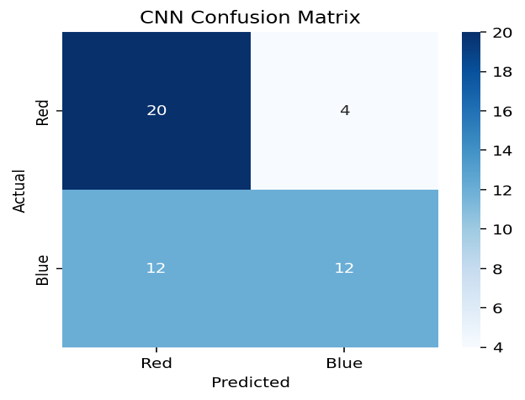
\includegraphics[width=0.5\linewidth]{image.png}
    \caption{Enter Caption}
    \label{fig:placeholder}
\end{figure}




During training all images captured under different environments have annotated real images. Combined with fly augmentation applied across 110 epochs, produced an effective training exposed into many image-labels seen by the model during training. The initial dataset split between training and test data caused unstable validation indicated the model required additional data. Once the model produced false negative and unreliable training rate based on observation of confusion matrix and split data between validation and testing required extra data, later added dataset applied a new setup for better progress.




 Models Reliability

The reliability rate implemented across iterative framework cycle in over 1200 collected images. During initial training stage the model classification increased only after multiple transformation based on previous failure. Despite the method seeming robust, however the detection confidence level remains volatile due to consistent transformation of the dataset combination. It was hard to comprehend the real cause as the model proved demanding systematic approach. Additional factor was that based on the nature of the model two colors representing solely dataset is not enough to deploy yolo for reliable model progress. The model is mainly compatible with large datasets. Despite expanding the dataset by applied all demanding approaches including lighting variations, position and background remain strongly dependent on datasets volume and diversity. In the middle of the model development process, it has been considered to introduce additional features to balance the dataset. Under tight assessment the additional features will contradicted with mechanical design. The latest new feature consideration was adding new rectangular or triangular boxes to extend the diversity of datasets since clearly behaved as Data-hungry architecture. The assessment was reached because the model clearly required large data which indicated the model relied heavily on extensive datasets. Preprocessing implemented different techniques to reduce noise and lighting normalization to improve detection accuracy.

Failure modes 

The model encountered multiple failures, dominated by misclassification under training stage. Lighting conditions have remained critical, specifically in low illumination around 160 lux. Under reduced illumination the training pipeline value threshold excluded the surface pixels on blue balls that measured brightness falls below minimum threshold. The condition outlined that despite the pipeline combined HSV and YOLOv8 failed to detect blue balls. Since the first method failed to achieve detection confidence, YOLOv8 architecture trained with brightness augmentation delivered more robust under the same low lighting level. Despite YOLOv8’s certain achievements still the model’s confidence score remained under low level of threshold 0.85 which indicated below agree 0.95 threshold. The fundamental problem was due to partly overlapping some balls with incomplete visual balls that complicated the detection ended up reducing confidence score.

Assessment of success and failure implemented across training and testing disciplines. The training detection success achieved to score reliable accuracy rate after multiple iterative attempts. The method to identify and mitigate failure was not comparable with test part. Under training phase failures are visible through confusion metric, validation accuracy that separated from training performance accuracy. It has been less complex to specify which color class with average precision fails to be assembled data. During model deployment failures are visible through the system’s behavior and analysis observed against the robot arm. The observation proved that the robot arm detected as perception system integrated, however not reached the right position in the first test. Another problem due to mechanical failure as the design of the arm which went through multiple print. Despite reliable training the arm misclassified, and the training metrics gave no warning about. This was the first observation that a model that trains reliable has failed at deployment for reasons that training metrics deliberately ignored.

During training, the neural network model by YOLOv detection architecture the model.

The model underwent through iterative training framework that improve to reach accuracy rate. During training epochs, the training loss significantly required continuous intervention before deployment consideration. The box regression loss, which measured how accurately the model is predicting bounding coordinates were frequently unstable values specifically on blue color. The classification loss was relatively stable, however did not bring valuable information due to the model clearly depending on random guessing. Despite the anticipated outcome the COCO trained resolved moved useful low-level features, the new classification. The yolo algorithm classification head predicts class probabilities for detecting bounding box after backbone to extract features At the beginning of training (epoch 0 ), the classification heads anticipated randomly initialized due to the model having not learned color representation. The consequence randomness demonstrated very low-level class confidence for the selected dataset. Despite consistent prediction localization the class probability did not transform because of failed learning new patterns. The confidence only increased after multiple epochs of supervised training based on labeled data 

Another isolated failure between 4 epochs that caused confusion for tangible analysis due to large loss fell from 8.6 into 3.2. The most significant reduction after some stable probabilities again falls in box regression. The detection head learned to use the pretrained edges and shape features to locate the circular boundary of each ball. The validation accuracy increases at Epoch 12, to 0.85 and 0.87 and at Epoch 18. This phase indicated the value of transfer learning, where backbone pertained learning accelerated merging and enables the detection images map detected the shapes ball classes. The performance outlined that useful progress supported by transfer learning with clear detection enhanced blue ball detection which balanced class performance and improved systems reliability. The statical model showed only after training multiple time scored effective confidence level due forget to be captured how the initial epoch demonstrated in fresh classification. 

 The resolution maintained to capture new additional images especially under circular light reflection with absence of balls, annotated empty files. Adding these empty files led the model to learn that blue shadows on the black belt are not balls. Training conducted by restart 

 Precision and Recall behavior under training.

Precision progress initially scored moderate level, however through training, and understanding these changes reveals how the model learning. During the initial epochs (1 to 24) the precision and Recall curve was diagonal at an exponential rate. The line from high precision at low to high recall at low precision. The model seems to have missed balls and is confident at same time during confidence threshold set high. This anticipated behavior stated that the model scores high confidence prediction only when evidence positive and certain. Another Epoch observation the curve shifted significantly where the precision remained high at recall level. The fact is the model reflected how learning progress developed. 


\begin{figure}
    \centering
    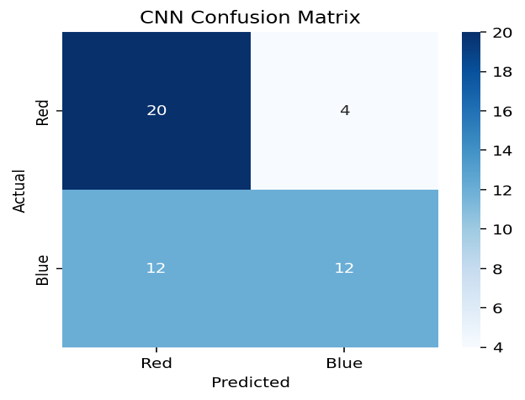
\includegraphics[width=0.5\linewidth]{image.png}
    \caption{Enter Caption}
    \label{fig:placeholder}
\end{figure}





The model learning detect balls seems reliable, while struggling with edge within the frame boundary. The balls under less lighting, and shadow blue. In final epoch stage the precision and recall curves. The model delivered high precision rate with limited epoch relatively positive prediction. Based on the confusion matrix the model submitted only three red balls incorrectly. The confusion matrix demonstrated the proposed classification achieved a precision 100 \%. This reflected the absence of false positive prediction for the red class. However, the recall value remained 87.5 \% stated that several red instances were misclassified that ended up in false negative. This behavior of the model suggested that model adopts conservative prediction including reliable prediction over detection sensitivity. The diagram showed the latest result where precision score precise target, while recall remain fragile 



 Despite the model scores 95 \% accuracy on held out test the failed in test stage. 

  These failures were only identified during initial integration test after the model deployed on the raspberry pi connected to the full system. Despite these failures were identified and corrected , however remain invisible due to did not appeared in reliable test metrics. These documented only because of it has been assumed that embedded in the training process that was not apparent until the model deployed in real environment.

 During model deployment test phase where the model integrated test grippe, two consecutive red and blue balls produced no detection output. The perception layer did not detect the YOLOv8 pipeline and routed the balls to the review bin. The confidence monitoring log indicated that YOLOv8 was generated a bounding box in the correct region with confidence 0.38 which far below from the actual 0. 70 threshold that did not reported as valid detection. The analysis indicated the images framed rom the two failed detections revealed that the sort area device(LED) loose the balls connection that caused.

The camera ms exposure time captured both limited and unlimited states, producing motion blur degradation in captured frames. This indicated the root cause might be the blue ball appear as green smear lacking the sharp edges and clear contours the YOLOv8 model depends on the for feature extraction and bounding box generation. Despite the model has trained on images with little motion blur , it ended up failed to confidently recognize the distorted balls caused detection failure.

After close inspection the model again retrain by build model resilience against  future issues 110 training images were augmented with simulated gaussian motion blur. Another measure fine-tuning has been apply where the model was fine-tuned for 24 epochs starting from the epoch 164 control point. The objective was to preserving previously learned features while adopting to motion blur data. The outcome after fine-tuning of the model confidence on the previously failed, motion blur frames increased to 0.87 demonstrated restored recognition , however it did not meet enough recognition ability. the observation revealed that detection failure caused by flashing motion blur were effective by combination of hardware repair and targeted data with motion blur simulation. This combined approach resolved and enhanced the models ability, however failed to generalized to all images. The perception layer of the robot arm could not recognized consistency that sensor indicated had less robust ability during sorting balls in real time. 

The difference of between training and deployment test 

The models validation evaluation metrics during training is not always reliable despite divers actual metric applied during evaluation phase. The difference between model assessment under training and in real time operation during  test performance scored distinct progress . This emphasized that tight comprehensive test required not only for systems behavior, but also support for systems specification review. This metric effectively measures of performance how the model progress generalized against train data. During test bin real time the model reveled a number of failures. In initial test blue color under dim lighting condition seen during training, while failed in real time by sensor system. These failure represent boundary that seems model prediction decreased a scenario that has never been visible during training stage. Many such weakness only visible during test in real time under partial integration.

  The model validation clearly underscored how the model believe to trained effectively and performed on the data that has been thought to collected, while test in a real time delivered how the model progressed in real operation. The MAP method seems valid and important metric for analysis model accuracy within the training distribution, it cannot predict how well a model perform  on the diverse, unpredictable inputs encountered in real time sort task. To achieve effective and reliable test output required diverse and incremental validation with integration test. This a fundamental method to address the models weakness beyond training boundaries and ensuring reliable result in real time deployment.







  
